\chapter{Analyse van Observatieprestaties}
\label{ch:analyse}

\section{Inleiding}

In de voorgaande hoofdstukken werden de ontwikkeling van de PoC applicatie, de methodologie voor het verzamelen 
van experimentele data, en het creëren van een grondwaarheidsdataset uitvoerig besproken. 
Dit hoofdstuk richt zich op de kern van het onderzoek: de geautomatiseerde analyse van de 
observatieprestaties van studenten aan de hand van de verzamelde eyetracking-opnames.

Het hoofddoel van de hier beschreven analyse is om, op basis van de videofeed en blikdata van de Tobii Pro Glasses 3, 
automatisch te bepalen (1) welke van de vooraf gedefinieerde kritische objecten door een student zijn waargenomen en (2) 
hoe lang de aandacht op elk van deze objecten gericht was. 
Om dit te realiseren, werd een analysepipeline ontworpen en geïmplementeerd, die de output van verschillende computervisiemodellen combineert.

De ontwikkelde analysepipeline, zoals conceptueel voorgesteld in Strategie 4 van Hoofdstuk~\ref{ch:oplossingsstrategieen}, 
transformeert de ruwe video- en blikdata frame per frame tot een identificatie van bekeken, kritische objecten. 
Dit proces omvat drie hoofdfasen: (1) het segmenteren en tracken van alle potentiële objecten in beeld, 
(2) het filteren van deze segmenten op basis van objectgrootte en daadwerkelijke observatie door de student, en 
(3) het classificeren van de overgebleven objectsegmenten. 
Er worden twee verschillende benaderingen voor de classificatiestap geëvalueerd: één op basis van image embeddings (DINOv2) en een vector-index (Faiss), 
en een tweede die gebruikmaakt van een getraind YOLO-classificatiemodel. 
De prestaties van deze methoden zullen worden beoordeeld aan de hand van de in Hoofdstuk~\ref{ch:grondwaarheid} gecreëerde grondwaarheid.

Figuur~\ref{fig:analyse-pipeline-visualisatie} illustreert de fasen van dit proces aan de hand van illustratieve beelden.

\begin{figure}[H]
    \centering
        \begin{subfigure}[b]{0.75\textwidth}
        \centering
        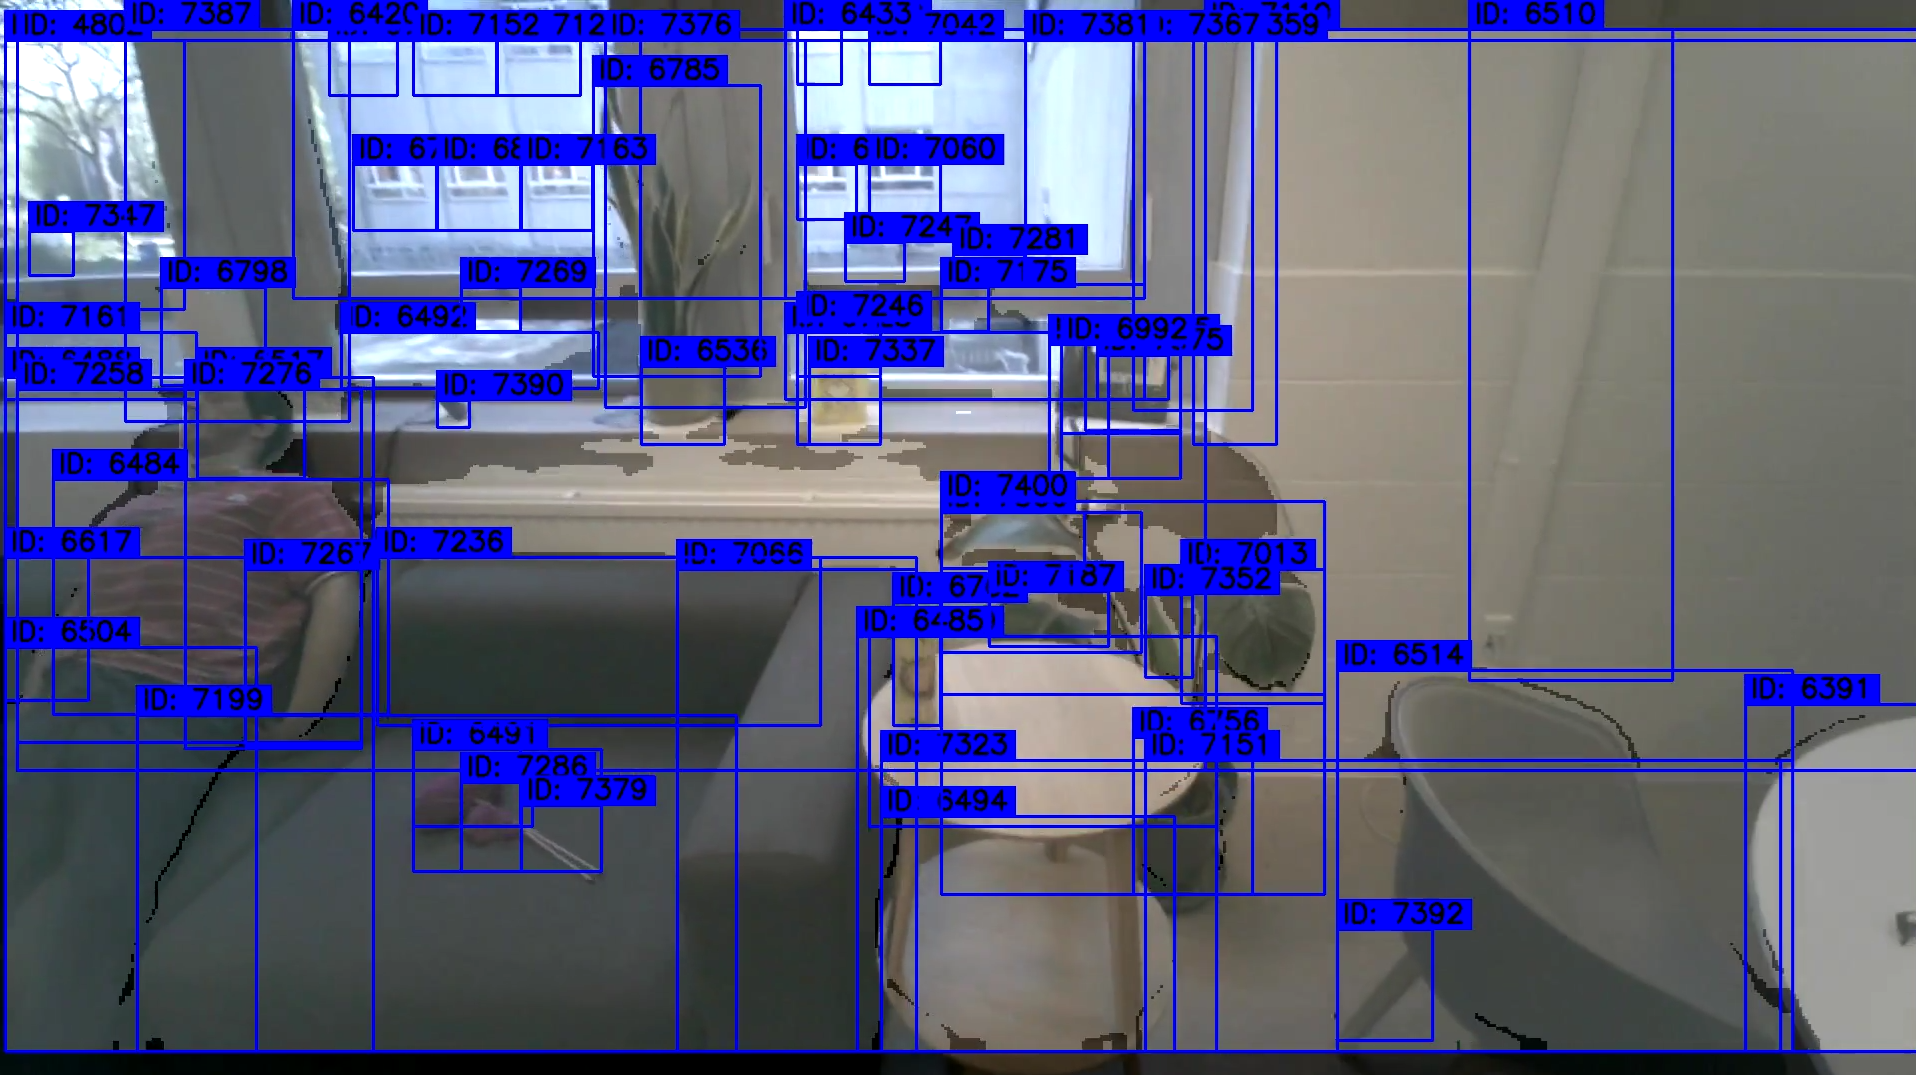
\includegraphics[width=1\textwidth]{everything-prompt.png}
        \caption{Everything-Segmentatie (FastSAM)}
        \label{fig:pipeline_stap_a}
    \end{subfigure}

    \vspace{0.5cm}

    \begin{subfigure}[b]{0.75\textwidth}
    \centering
    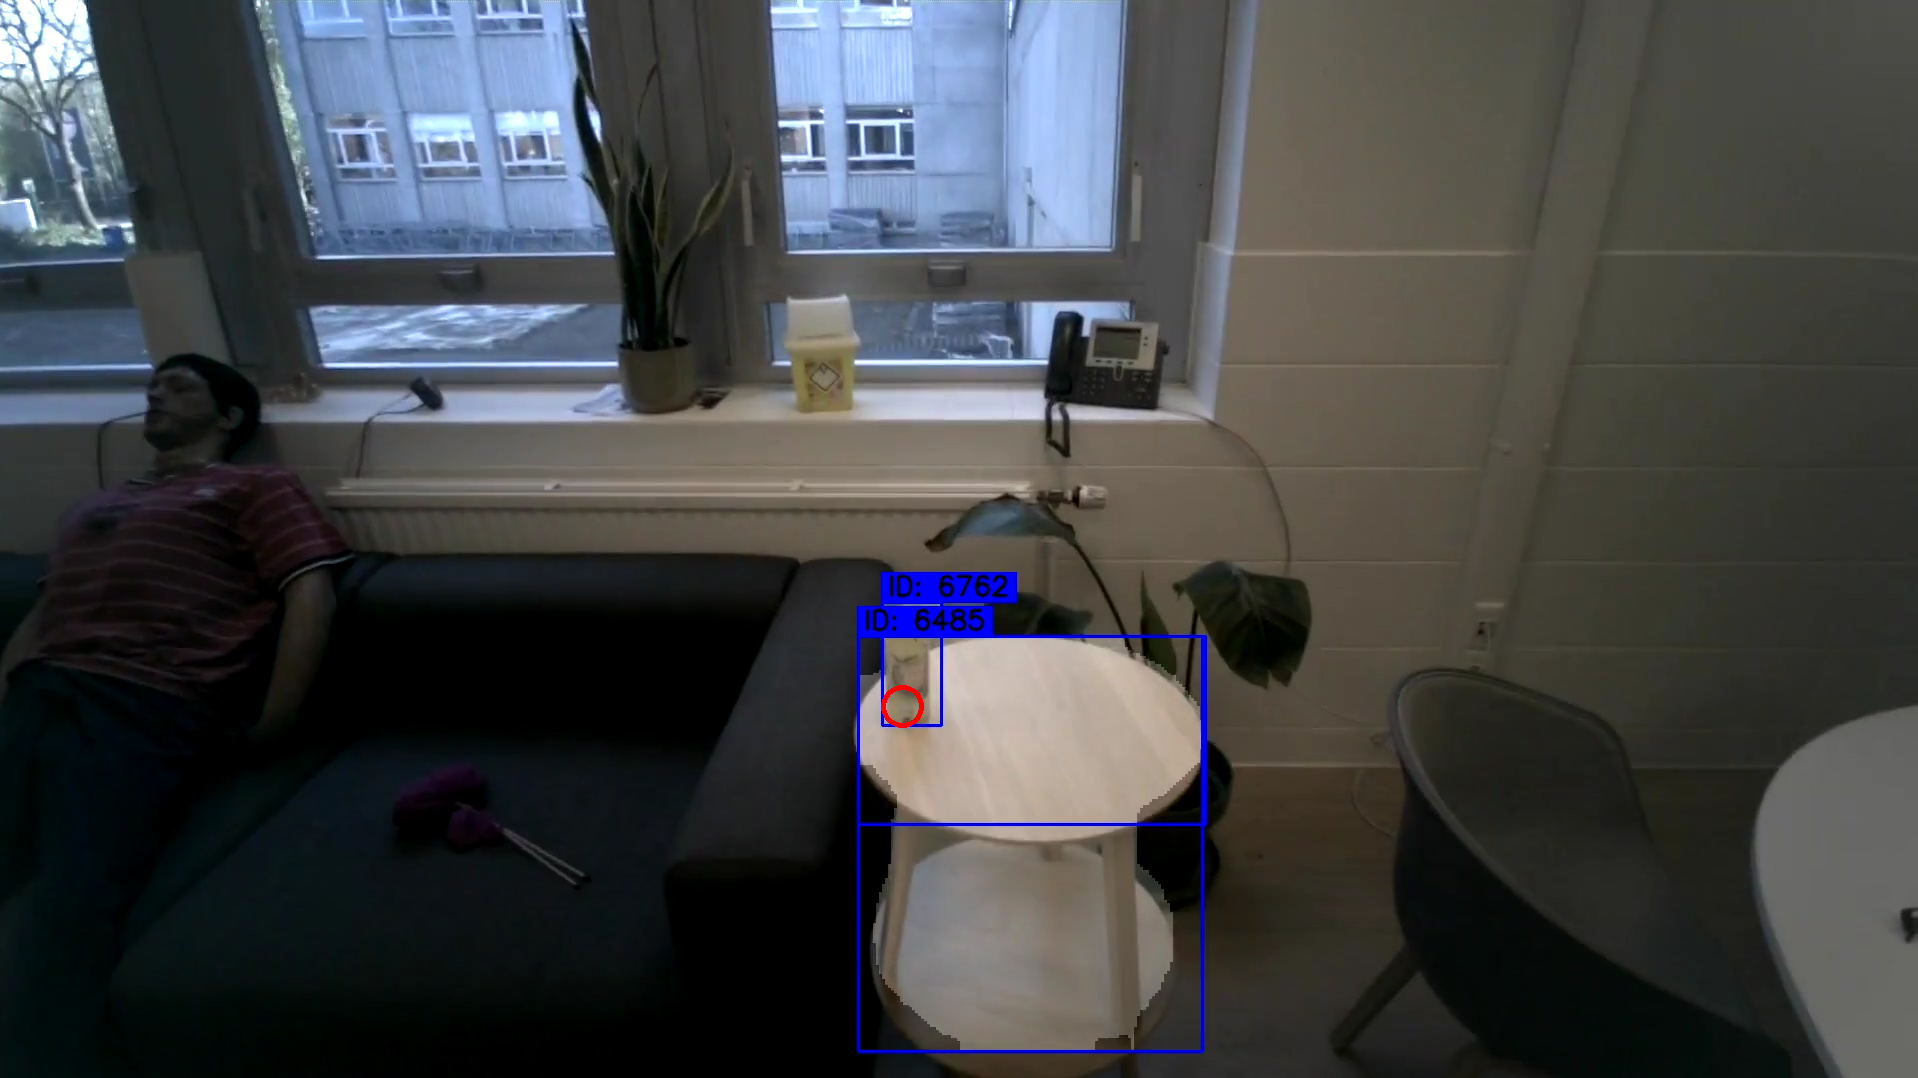
\includegraphics[width=1\textwidth]{filtered-segmentation.png}
    \caption{Filtering op basis van blikpunt en objectgrootte}
    \label{fig:pipeline_stap_b}
    \end{subfigure}

    \vspace{0.5cm}

    \begin{subfigure}[b]{0.75\textwidth}
        \centering
        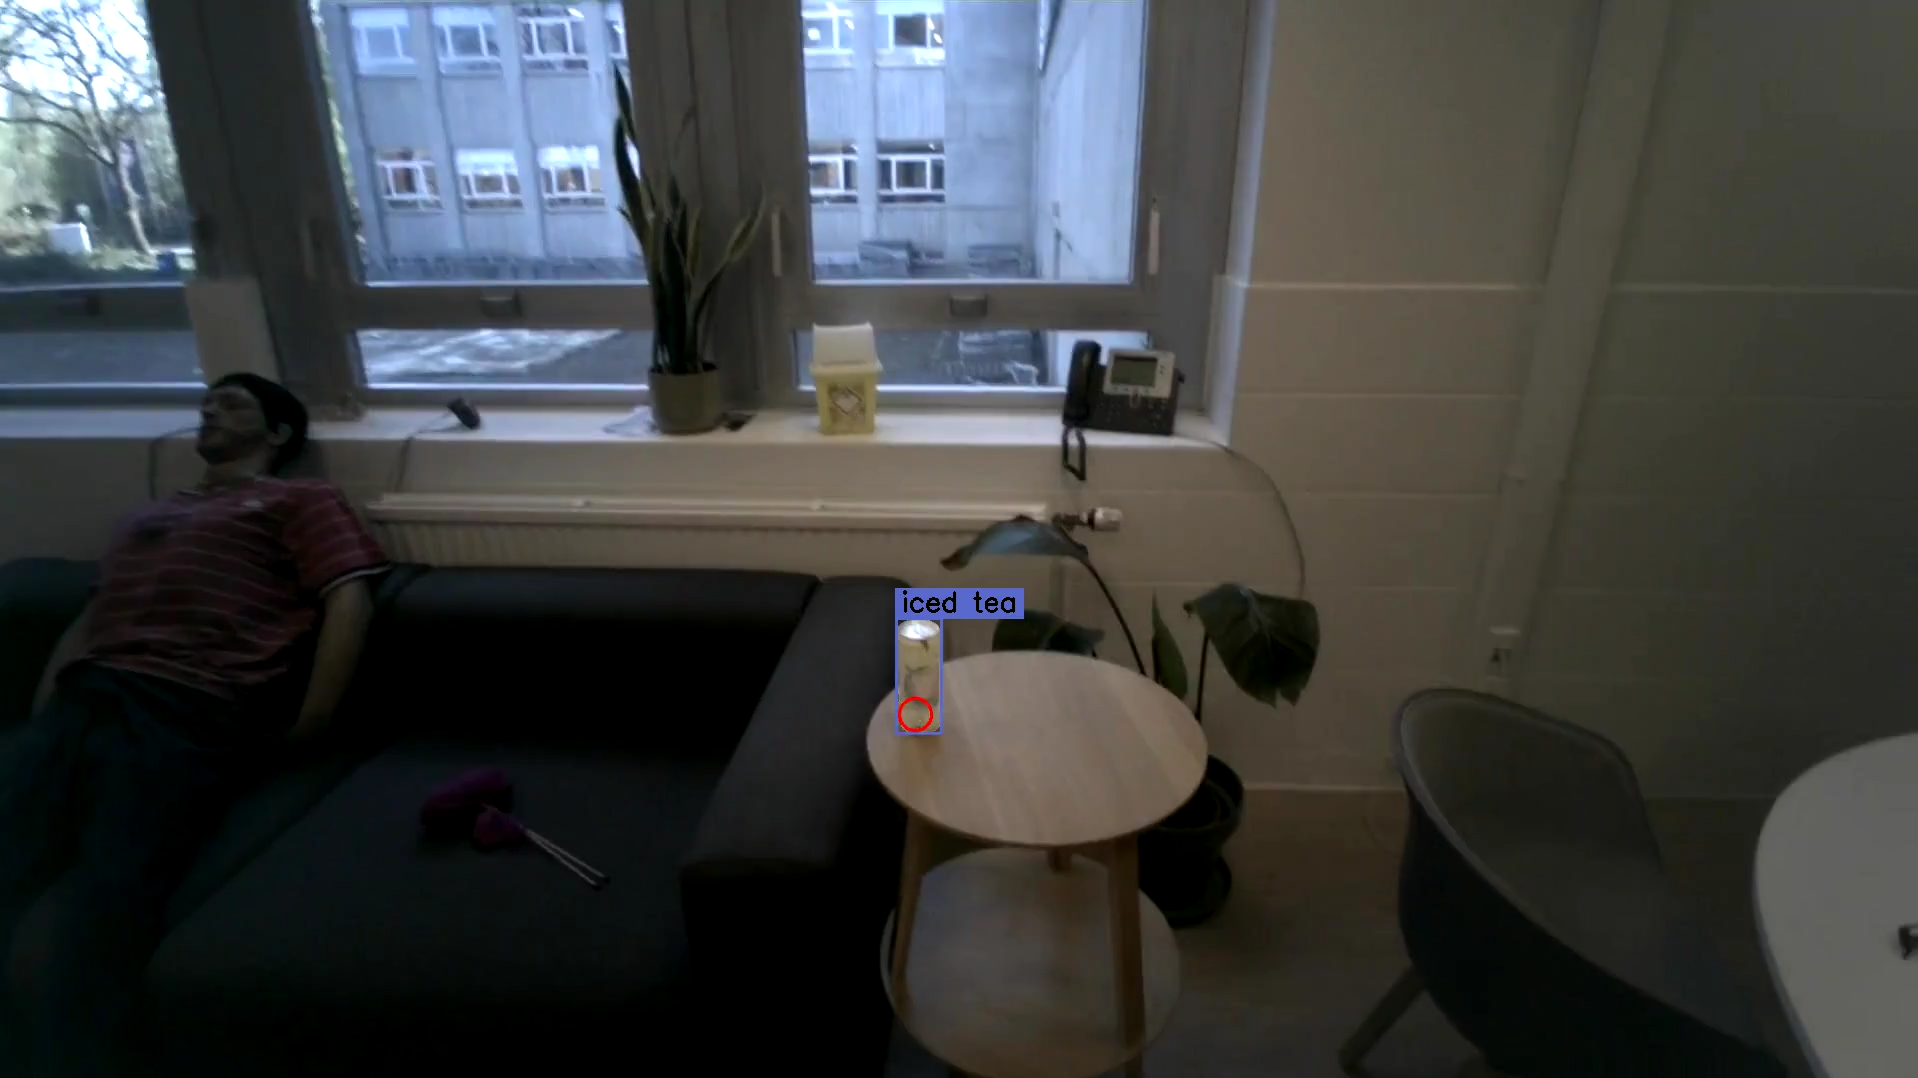
\includegraphics[width=1\textwidth]{classification-example.png}
        \caption{Classificatiestap*}
        \label{fig:pipeline_stap_c}
    \end{subfigure}
    \caption[Visualisatie van de Analysepipeline]{
        \label{fig:analyse-pipeline-visualisatie}
        Visualisatie van de stappen in de analysepipeline.
        (\subref{fig:pipeline_stap_a}) FastSAM identificeert en segmenteert alle potentiële objecten in het frame.
        (\subref{fig:pipeline_stap_b}) De segmenten worden gefilterd; enkel de segmenten die daadwerkelijk met de blik van de gebruiker overlappen worden behouden.
        (\subref{fig:pipeline_stap_c}) De overgebleven segmenten worden uit de originele frame geknipt en dienen als input voor een classificatiemodel.
        *De afbeelding voor de classificatiestap in dit voorbeeld is afkomstig uit een labeling-validatie video.
    }
\end{figure}

\section{Everything-Segmentatie en Objectfiltering}

De eerste fase van de analysepipeline is erop gericht om uit de continue videostroom alle potentieel relevante objectregio's 
te isoleren die daadwerkelijk door de student zijn bekeken. 
De implementatie van dit proces werd vastgelegd in de python-notebook \texttt{04\_gaze\_segmentation.ipynb},
en wordt hieronder toegelicht.
Alle besproken code is te vinden binnen de \texttt{GazeSegmentationJob} klasse in de notebook.

\subsection{Tracking en Segmentatie met FastSAM}

Het FastSAM-model komt in twee varianten: een `large' (\texttt{FastSAM-x}) en een `small' (\texttt{FastSAM-s}) versie.
Hier werd gekozen om de `large' versie te gebruiken, vanwege de betere prestaties in termen van segmentatie en tracking.
Dit model is beschikbaar via de \texttt{ultralytics}\footnote{\url{https://docs.ultralytics.com/models/fast-sam/}} python-bibliotheek,
en bevat een \texttt{track} functie die het mogelijk maakt om alle objecten in een video zowel te segmenteren als te tracken.

\subsubsection{Tracking en Segmentatie van Objecten}

In een eerste stap worden alle frames van de evaluatieopname geëxtraheerd naar een tijdelijke map met behulp van \texttt{ffmpeg}.
Daarna is het mogelijk om de \texttt{track} functie aan te roepen op deze frames:

\begin{listing}[H]
  \begin{minted}{python}
    frame_paths = list(self.frames_path.iterdir())
    # Frames sorteren op basis van hun naam (index)
    frame_paths.sort(key=lambda x: int(x.stem))

    for frame_path in frame_paths:
        frame_idx = int(frame_path.stem)
        results = self.model.track(
            source=str(frame_path), imgsz=1024, verbose=False, persist=True
        )[0]
    \end{minted}
  \caption[Tracking van objecten met FastSAM]{}
\end{listing}

Hier zijn volgende zaken belangrijk om op te merken:
\begin{itemize}
    \item De frames dienen gesorteerd te worden op basis van hun volgorde in de video.
    \item De \texttt{track} functie neemt een parameter \texttt{imgsz} aan, die de grootte van de inputafbeeldingen bepaalt.
    Indien de afbeeldingen te groot of te klein zijn, worden ze automatisch geschaald.
    Deze parameter heeft zowel invloed op de snelheid van de segmentatie als op de kwaliteit ervan.
    \item Het is belangrijk om de \texttt{persist} parameter op \texttt{True} te zetten, 
    zodat het model de tracking-informatie kan behouden tussen opeenvolgende frames.
    \item De \texttt{track} functie retourneert een lijst van \texttt{Results}-objecten maar bevat hier slechts één element.
    Dit \texttt{Results}-object bevat de segmentatiemaskers, bounding boxes, en tracking-informatie voor elk object in het frame.
\end{itemize}

\subsubsection{Filteren van Tracking-Resultaten}

% TODO: wat doen met frames waar geen gazedata is? (objecten kunnen nog steeds nuttig zijn voor classificatie binnen een object-id)

Na het uitvoeren van de tracking en segmentatie, worden de resultaten gefilterd op basis van twee criteria:
\begin{itemize}
    \item \textbf{Objectgrootte:} Segmenten die een onrealistisch groot deel van het beeld beslaan (bijvoorbeeld muren, vloeren, of de gehele achtergrond) worden weggelaten.
    \item \textbf{Blikdata:} Met behulp van de \texttt{mask\_was\_viewed} functie (zie Sectie~\ref{sec:omgaan-met-blikdata}) 
    wordt voor elk overgebleven segment gecontroleerd of het blikveld van de student daadwerkelijk overlapt met het segmentatiemasker in dat specifieke frame. 
    Enkel de `bekeken' segmenten worden behouden voor verdere analyse.
\end{itemize}

Aangezien we het al eerder hebben gehad over de \texttt{mask\_was\_viewed} functie, 
zal hier enkel de \texttt{mask\_too\_large} functie worden besproken:

\begin{listing}[H]
  \begin{minted}{python}
    def mask_too_large(self, mask: torch.Tensor) -> bool:
        MAX_MASK_AREA = 0.1
        height, width = mask.shape
        frame_area = height * width
        max_mask_area = MAX_MASK_AREA * frame_area

        mask_area = mask.sum()
        return mask_area >= max_mask_area
    \end{minted}
  \caption[Filteren van segmenten op basis van grootte]{}
\end{listing}

Hier wordt een som berekend van alle pixels in het segmentatiemasker (aangezien het masker binair is).
Indien deze som groter is dan de maximaal toegestane oppervlakte, wordt het masker als `te groot' beschouwd.
De maximale oppervlakte van een segment wordt gedefinieerd als 10\% van de totale oppervlakte van het frame.
Dit is momenteel een arbitraire waarde, maar kan in de toekomst verder geoptimaliseerd worden, of zelfs 
dynamisch worden ingesteld op basis van objecten binnen kalibratieopnames in de applicatie.

\subsubsection{Opslaan van de Resultaten}

Na het filteren van de segmenten, worden de resultaten opgeslagen in gecomprimeerde numpy-bestanden 
(\texttt{.npz}) onder \texttt{data/gaze\_segmentation\_results}.

\begin{listing}[H]
  \begin{minted}{python}
    executor.submit(
        np.savez_compressed,
        self.results_path / f"{frame_idx}.npz",
        boxes=boxes,
        rois=rois_array,
        masks=masks_array,
        object_ids=object_ids,
        frame_idx=frame_idx,
        gaze_position=gaze_position,
        confidences=confidences,
    )
    \end{minted}
  \caption[Opslaan van segmentatie-resultaten]{}
\end{listing}

De volgende gegevens worden opgeslagen:
\begin{itemize}
    \item \textbf{boxes:} De bounding boxes van de segmenten, handig voor het visualiseren van de segmenten in de video.
    \item \textbf{rois:} De ROI's (Region of Interest) van de segmenten. Deze worden later gebruikt bij de classificatiestap om de objecten te identificeren.
    \item \textbf{masks:} De segmentatiemaskers van de objecten, die ook worden gebruikt voor visualisatie.
    \item \textbf{object\_ids:} De unieke ID's van de objecten, die worden toegewezen door het FastSAM-model.
    \item \textbf{frame\_idx:} De index van het frame, die wordt gebruikt om de resultaten te koppelen aan het juiste frame in de video.
    \item \textbf{gaze\_position:} De blikpositie van de student in dat specifieke frame.
    \item \textbf{confidences:} De vertrouwensscore van het model voor elk segment, die aangeeft hoe zeker het model is dat het segment correct is.
    Dit kan nuttig zijn voor het filteren van segmenten die een lage vertrouwensscore hebben, 
    of het vinden van correlaties tussen de vertrouwensscore en de uiteindelijke classificatie.
\end{itemize}
Aangezien het opslaan van de resultaten IO-intensief is, wordt dit proces uitgevoerd met behulp van multithreading.

\section{Classificatie van Objecten}

\subsection{Voorbereiding van Data voor Classificatie}

De output van de voorgaande fase bestaat uit een reeks \texttt{.npz}-bestanden, één per frame, 
die de gefilterde segmenten, ROIs, en bijbehorende metadata bevatten. 
Om deze data efficiënt te kunnen gebruiken als input voor de classificatiestrategieën, werd een aanvullende voorbereidingsstap uitgevoerd. 
Deze stap werd geïmplementeerd in de notebook \texttt{05\_create\_object\_datasets.ipynb} en consolideert de frame-per-frame 
resultaten tot een gestructureerde dataset per evaluatieopname. 
Deze dataset, hierna "object-dataset" genoemd, vormt de directe input voor zowel de classificatie met een vector-index als de 
classificatie met een YOLO-model.

Het creëren van de object-dataset omvat het itereren over de \texttt{.npz}-bestanden van elke opname. 
Voor elk gedetecteerd en gefilterd object (ROI) binnen een frame worden de volgende kenmerken geëxtraheerd en samengevoegd:
\begin{itemize}
    \item \texttt{frame\_idx}: De index van het frame waarin het object oorspronkelijk werd gedetecteerd. 
    Dit koppelt het object aan een specifiek tijdstip in de video.
    \item \texttt{object\_id}: De unieke, tijdelijke ID die door het FastSAM-model aan het getrackte object 
    is toegewezen binnen de scope van die specifieke tracking-sessie.
    \item \texttt{confidence}: De confidencescore van het FastSAM-model voor de detectie van dit specifieke segment. 
    Deze score geeft een indicatie van hoe zeker het model was van zijn segmentatie.
    \item \texttt{embedding}: Een dense vectorrepresentatie (embedding) van de visuele kenmerken van de ROI, 
    gegenereerd met het DINOv2-model. 
    Deze embedding dient als input voor de op similariteit gebaseerde classificatie met een vector-index.
    Meer hierover in de sectie dat volgt.
    \item \texttt{mask\_area}: De totale oppervlakte van het segmentatiemasker van het object in pixels. 
    Dit geeft een maat voor de (schijnbare) grootte van het object in het frame.
    \item \texttt{x1, y1, x2, y2}: De coördinaten die de bounding box rondom het gedetecteerde object definiëren. 
\end{itemize}

Deze geëxtraheerde informatie wordt per opname samengevoegd in een \texttt{Pandas DataFrame} en vervolgens opgeslagen 
als een \texttt{.csv}-bestand onder \texttt{data/object\_datasets/<recording\_id>}. 
Het resultaat is een set van tabelvormige datasets die klaar zijn voor de daadwerkelijke classificatietaken.
Hoewel veel van deze metadata ook in de individuele \texttt{.npz}-bestanden te vinden is, resulteert de consolidatie 
naar één \texttt{.csv}-bestand per opname in een efficiëntere dataverwerking tijdens de classificatiefase. 
Het vermijdt het herhaaldelijk openen en parsen van potentieel honderden of duizenden afzonderlijke \texttt{.npz}-bestanden

\subsection{Classificatie met Vector-Index}

\subsection{Classificatie met YOLO}

